\documentclass[11pt]{article}
\usepackage[a4paper,margin=24mm]{geometry}
\usepackage[T1]{fontenc}
\usepackage{lmodern}
\usepackage{amsmath,amssymb,bm,booktabs}
\usepackage{graphicx}
\usepackage{subcaption}
\usepackage{xcolor}
\definecolor{referenceblue}{RGB}{25,55,95}
\usepackage[colorlinks=true,linkcolor=referenceblue,citecolor=referenceblue,urlcolor=referenceblue]{hyperref}
\setlength{\parindent}{1.4em}
\setlength{\parskip}{2pt}
\setlength{\textfloatsep}{14pt}
\newcommand{\qmix}{q_{\!K}}
\newcommand{\dd}{\mathrm{d}}
% BEGIN AUDITED DATA: populated by sync_manuscript_data.py
% Snapshot: cfdf0f110010d688a4e3c48f6d88a00fd17dc698; no P24 physical data.
% Evidence JSON SHA256: db7c5908e2cad5c749c7914f4eb742b28d1d404b4124a03107f35b94ad013bd3
\newcommand{\PlateAMM}{300}
\newcommand{\PlateBMM}{100}
\newcommand{\HoleCxMM}{170}
\newcommand{\HoleCyMM}{-20}
\newcommand{\HoleRMM}{30}
\newcommand{\PhiStar}{-1.5606}
\newcommand{\MouthX}{0.199989}
\newcommand{\MouthY}{-0.0208170}
\newcommand{\NormalX}{0.999629}
\newcommand{\NormalY}{-0.0272345}
\newcommand{\PeakStress}{3.7141}
\newcommand{\LoadFactor}{80.774}
\newcommand{\LastXMM}{291.840}
\newcommand{\LastYMM}{-25.579}
\newcommand{\LSLengthMM}{84.15}
\newcommand{\LastLigamentMM}{8.16}
\newcommand{\MinimumTheta}{-3.646}
\newcommand{\MaxCODError}{0.01024}
\newcommand{\CODQuadMin}{0.6204}
\newcommand{\CODQuadMax}{0.6225}
\newcommand{\CODNearZeroPercent}{26.3}
\newcommand{\CODNearZeroTurnDiff}{0.00245}
\newcommand{\SyntheticRelativeError}{3.86\times10^{-8}}
\newcommand{\MaxTrueResidual}{1.00\times10^{-10}}
\newcommand{\CharacteristicRows}{$P_{1}$ & 4 & 0.36648 & $4.198\times10^{-6}$ & $1.146\times10^{-5}$ & 0.0000 & -0.00131 \\
$P_{17}$ & 68 & 0.78679 & $2.548\times10^{-3}$ & $3.239\times10^{-3}$ & -2.4444 & -0.37115 \\
$P_{21}$ & 84 & 0.96631 & $7.860\times10^{-5}$ & $8.134\times10^{-5}$ & -3.6366 & -0.00932 \\
$P_{22}$ & 88 & 1.0667 & $-2.284\times10^{-3}$ & $-2.142\times10^{-3}$ & -3.6460 & +0.24541 \\
$P_{23}$ & 92 & 1.2444 & $-6.780\times10^{-3}$ & $-5.449\times10^{-3}$ & -3.4006 & +0.62435 \\}
% END AUDITED DATA
\title{Incremental LEFM Prediction of a Crack Trajectory\\from a Circular Hole}
\author{}
\date{}

\begin{document}
\maketitle
\begin{abstract}
Crack-direction prediction from a circular hole is examined as a recursively
coupled numerical problem in quasi-static linear elastic fracture mechanics.
The initiation point is selected from the maximum tensile tangential stress
on the uncracked hole boundary. An initial segment follows its material-side
normal, and subsequent directions are obtained from current-tip opening and
sliding stress-intensity factors through the maximum tangential stress
criterion. Each elastic solution retains the previously generated crack
geometry. Reflection-paired tip meshes, prescribed-field extraction checks,
independent crack-opening-displacement comparisons, and a centered-hole
control support the numerical assessment. Fixed-geometry mesh comparisons
and independently propagated mesh and increment studies distinguish
extraction sensitivity from accumulated trajectory sensitivity. Mode mixity
first increases and then changes sign as the crack develops, reversing the
incremental turn while the opening intensity continues to increase.
Characteristic path events persist under the tested mesh changes, while
increment refinement contracts geometric and directional discrepancies and
retains stable increment-normalized turning measures. These observations
support numerical robustness within the tested families, rather than a
rigorous error bound or a uniquely established boundary mechanism. The
model addresses direction selection under prescribed increments; it does
not resolve propagation kinetics, arrest, branching, or inelastic processes.
\end{abstract}
\noindent\textbf{Keywords:} crack trajectory; circular hole; linear elastic
fracture mechanics; maximum tangential stress; mode mixity; interaction
integral; crack-opening displacement.

\section{Introduction}
Circular holes are among the classical stress concentrators of fracture
mechanics.  Once a crack is prescribed at a hole boundary, its stress-
intensity factors have been studied analytically for radial and inclined
configurations since the early work of Bowie~\cite{Bowie1956}; mixed-mode
solutions for cracks emanating from circular holes were subsequently
developed for finite plates~\cite{WooWangCheung1989}, and modern
weight-function formulations provide efficient mixed-mode SIF and
crack-opening-displacement estimates for hole-edge cracks~\cite{XuEtAl2018}.
The onset problem is related but distinct.  Finite-fracture-mechanics
studies have examined crack initiation from an initially uncracked circular
hole, including the competition between symmetric and asymmetric
initiation~\cite{SaporaEtAl2018} and the stability of subsequent growth
under biaxial loading~\cite{SaporaCornetti2018}.  These results emphasize
a basic distinction that is central here: identification of an initiation
site does not by itself determine the trajectory of the finite crack that
subsequently develops.

Once a finite crack exists, its direction depends on the mixed-mode field
at its current tip and therefore on the complete crack geometry accumulated
up to that state.  The maximum tangential stress (MTS) criterion of Erdogan
and Sih~\cite{ErdoganSih1963} provides a classical local direction rule in
terms of the opening and sliding intensities $K_I$ and $K_{II}$,
respectively. Numerical crack-growth frameworks have long
combined such local criteria with repeated updating or remeshing of the
geometry; for example, Bouchard et al.~\cite{BouchardEtAl2003} compared
several mixed-mode direction criteria within an automatic finite-element
propagation procedure.  At a different modeling scale, cohesive-zone
formulations replace the singular-tip idealization by a finite fracture
process zone.  Recent potential-based cohesive calculations in a near-LEFM
regime show that the selected kink direction can remain close to the
classical elastic prediction even when the critical load is more sensitive
to the cohesive-zone description~\cite{BogdanovSelivanov2026}.  The
present work deliberately remains within LEFM in order to isolate the
trajectory-selection problem itself.

Crack trajectories influenced by holes have been predicted using several
different numerical and semi-analytical technologies.  Wang et
al.~\cite{WangMeguidPapanikos1999} treated curved cracks emanating from
adjacent holes and compared predicted paths with fatigue experiments.
Boundary-element propagation has been used for multiple cracks in perforated
domains~\cite{LiuLiXie2017}, while Fang et al.~\cite{FangEtAl2020}
combined adaptive extended isogeometric analysis with an interaction
integral and the maximum circumferential-stress criterion for cracks
interacting with arbitrary holes and voids.  Their study also compared two
prescribed crack-growth increments and found similar trajectories, with the
smaller increment producing the smoother path.  Yang et
al.~\cite{YangEtAl2020} used incremental remeshing to study cracks
emanating from circular blasting holes and showed that, in mixed-mode
configurations, the sign and magnitude of $K_{II}$ govern the direction of
curving.  Related perforated-plate problems have been studied with a
boundary-cracklet formulation~\cite{AhmedEtAl2021}, and commercial
adaptive remeshing has been used to reproduce hole-induced crack deflection
and arrest~\cite{AlshoaibiFageehi2022}.  Taken together, these studies
establish both the strong physical influence of holes on crack paths and
the ability of several numerical technologies to reproduce such
interactions.

For an incremental trajectory calculation, however, the stress-intensity
factors are not merely postprocessed outputs.  They determine the next
segment, perturbing each later boundary-value problem.  Numerical
SIF extraction therefore enters the propagation algorithm recursively.
The mixed-mode interaction-integral construction provides a natural
energetic route to separating $K_I$ and $K_{II}$~\cite{YauWangCorten1980}.
Independent accuracy studies have shown that near-tip discretization and
postprocessing choices can materially affect extracted SIFs:
displacement-extrapolation estimates depend on element size, shape, and
mesh arrangement~\cite{GuineaPlanasElices2000}; energetic/domain-integral
approaches are generally less dependent on detailed near-tip field fitting
and are attractive for stepwise crack-growth calculations
\cite{CourtinEtAl2005}; and comparative studies report their best
finite-element SIF accuracy when domain integrals are combined with
appropriately refined meshes~\cite{QianEtAl2016}.  Ghafoori Ahangar and
Verreman~\cite{GhafooriAhangarVerreman2019} further demonstrated the
relative robustness of the interaction-integral method with respect to
angular discretization, element size, local refinement, crack length, and
mixed-mode extraction.  These results motivate treating verification of the
SIF calculation as part of the crack-path problem rather than as an
independent implementation detail.

The studies above provide extensive evidence for individual components of
incremental LEFM propagation, but comparatively less attention has been
given to the trajectory as a recursively generated numerical object whose
characteristic events should remain stable under controlled perturbations
of the numerical procedure.  The purpose of the present study is therefore
not to introduce a new mixed-mode fracture criterion or a new remeshing
technology.  Instead, we construct a single crack trajectory from a circular
stress concentrator and ask which features of that trajectory can be
regarded as robust consequences of the evolving elastic field.  The
uncracked-hole solution selects the initiation point and a material-side
normal; only the first crack segment is prescribed along that normal.
Every subsequent direction is obtained from the current-tip $K_I$ and
$K_{II}$ values through the MTS rule after solving the complete current
crack geometry.

The numerical assessment separates extraction accuracy from the sensitivity
of a recursively generated trajectory.  The interaction integral in equivalent domain form (EDI) is checked
against prescribed asymptotic fields and independent crack-opening-
displacement estimates.  A centered-hole control tests whether the same
EDI--MTS recurrence preserves and restores the exact straight symmetry
path.  Exterior-mesh density is perturbed independently, while a separate
structured-tip resolution study varies the near-tip scale while holding the
requested exterior sizing law fixed.  Finally, crack-increment sensitivity is examined through independently
generated 4-, 2-, and 1-mm paths using one dimensionless numerical family.
Particular attention is paid to the evolution of the mode mixity
$K_{II}/K_I$, the location of its positive maximum and sign reversal, the
corresponding change in turning sense, and the behavior of increment-
normalized corrective quantities.  This structure is intended
to distinguish a physically interpretable trajectory from one that is only
visually plausible within a particular discretization.

The contribution is a reproducible assessment of how initiation selection,
current-tip extraction, and prescribed increments interact during recursive
direction selection using established LEFM and MTS methods.
Section~\ref{sec:problem} defines the geometry, loading, and stress-selected
initiation frame. Section~\ref{sec:recurrence} develops the current-tip
directional recurrence. Section~\ref{sec:numerics} describes discretization,
extraction, and verification, and Section~\ref{sec:results} presents the
trajectory and sensitivity results. Section~\ref{sec:discussion} separates
the mechanical interpretation from discretization evidence and model
limitations. Section~\ref{sec:conclusions} summarizes the findings; the
supplementary diagnostics document numerical acceptance.

\section{Problem formulation}
\label{sec:problem}
\subsection{Geometry, material, and loading}
Figure~\ref{fig:geometry-loading} introduces the plate geometry, the
coordinate conventions, and the applied loading. The specimen has
width $2A$ and height $B$, with a circular hole of radius $R$ whose
center is denoted by $(x_c,y_c)$ in the schematic. The figure measures
$y_c$ upward from the lower plate edge. For the computational
formulation we use a Cartesian frame with origin at the midpoint of
the left edge, $x$ pointing right and $y$ upward. Thus
\[
  \Omega_{\mathrm{rect}}=[0,2A]\times[-B/2,B/2],
  \qquad (x_c,y_c^{\mathrm{comp}})=(x_c,y_c-B/2).
\]
The curved line emerging from the hole illustrates an admissible
crack path; it is schematic and does not prescribe the computed
trajectory. The initiation point $P_0$ is selected from the
uncracked-hole solution, and only the first crack direction is
prescribed. Subsequent directions follow from the current-tip SIFs.

% Figure environment maintained inline in main.tex; graphics remain separate PDFs.
\begin{figure}[htbp]
  \centering
  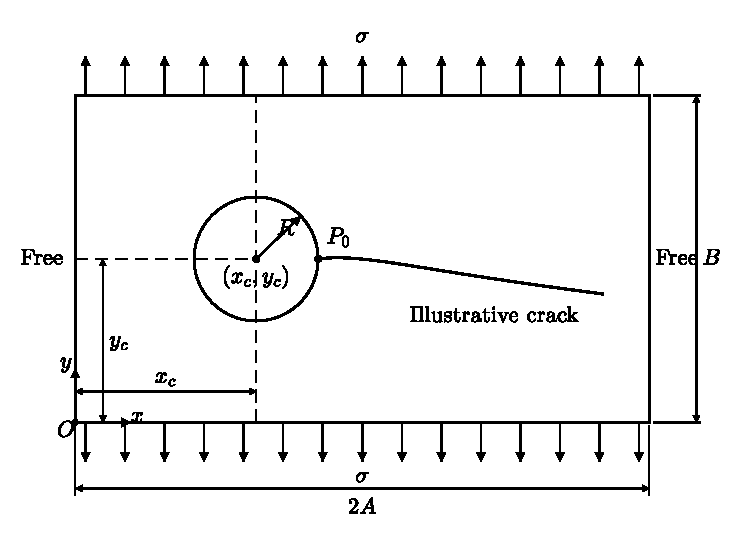
\includegraphics[width=0.78\textwidth]{figures/geometry_loading/specimen_geometry.pdf}
  \caption{Specimen geometry and tensile loading. The plate has width $2A$
  and height $B$, and the circular hole has radius $R$ and center
  $(x_c,y_c)$ in the schematic's lower-left coordinate system. The
  computational $y$ coordinate is shifted by $-B/2$ relative to the sketch.
  The symbolic sketch is not drawn to the numerical scale.
  The arrows indicate outward tensile tractions of unsigned magnitude
  $\sigma$; the lateral edges, hole boundary, and crack faces are
  traction-free. The curvilinear crack is schematic, not a prescribed or
  independently solved trajectory.}
  \label{fig:geometry-loading}
\end{figure}

At step $k$, $\Omega_k$ is the material domain outside the hole and the
retained crack $\Gamma_k$, with distinct upper and lower crack faces.
The material is homogeneous, isotropic, and linearly elastic,
with Young's modulus $E$ and Poisson's ratio $\nu$, under plane
strain. For the crack geometry $\Gamma_k$ ending at $P_k$, the
displacement field $\bm u$, strain tensor $\bm\varepsilon$, and stress
tensor $\bm\sigma$ satisfy
\begin{align}
 \nabla\!\cdot\bm{\sigma}&=\bm0 &&\text{in }\Omega_k,\label{eq:equilibrium}\\
 \bm{\varepsilon}&=\tfrac12(\nabla\bm u+\nabla\bm u^{\mathsf T}),\qquad
 \varepsilon_{33}=0,\label{eq:strain}\\
 \bm{\sigma}&=2\mu\bm{\varepsilon}
       +\lambda\,\operatorname{tr}(\bm{\varepsilon})\bm I,
 \quad \mu=\frac{E}{2(1+\nu)},\quad
 \lambda=\frac{E\nu}{(1+\nu)(1-2\nu)}.\label{eq:constitutive}
\end{align}
Here $\bm I$ is the identity tensor, and $\mu$ and $\lambda$ are the
shear modulus and first Lam\'e coefficient, both with stress units.
Uniform outward tensile tractions act on the horizontal edges, in the
directions indicated by the arrows in Fig.~\ref{fig:geometry-loading}.
Their unsigned magnitude is $\sigma>0$, as in the drawing. The traction
vectors on the upper and lower edges are $(0,\sigma)$ and
$(0,-\sigma)$, respectively. The vertical sides, hole boundary, and
crack faces are traction free. Rigid-body motions are removed by imposing
$u_x=u_y=0$ at the lower-left corner and $u_y=0$ at the lower-right
corner. There are no body forces.

For fixed geometry, positive scaling of $\sigma$ scales both SIFs
equally, preserving their ratio and the MTS direction. The present
formulation predicts the direction of imposed quasi-static increments,
not a load-versus-time crack-growth history.

\subsection{Stress-selected initiation and the frozen frame}
The uncracked-hole elastic field supplies the tangential boundary stress
$\sigma_{tt}(\phi)$, where $\phi$ is measured counterclockwise from the
positive Cartesian $x$ direction. Its maximum tensile value selects the
initiation point; the numerical boundary evaluation is described in
Section~\ref{sec:numerics}. Let $\sigma_c$ denote the tensile
initiation threshold. The dimensionless initiation multiplier
$\lambda_{\mathrm{ini}}$ is distinct from the Lam\'e coefficient $\lambda$.
The normalized initiation rule is
\begin{equation}
 \phi_* = \mathop{\operatorname{arg\,max}}_\phi
      \sigma_{tt}^{+}(\phi;\sigma),\qquad
 \lambda_{\mathrm{ini}}=
      \frac{\sigma_c}{\max_\phi\sigma_{tt}^{+}(\phi;\sigma)},
 \quad \sigma_{tt}^{+}=\max(\sigma_{tt},0).\label{eq:initiation}
\end{equation}
The fitted angle $\phi_*$ specifies the initiation point and the
outward material-side radial normal:
\begin{equation}
 P_0=\begin{bmatrix}x_c+R\cos\phi_*\\
                     y_c^{\mathrm{comp}}+R\sin\phi_*
     \end{bmatrix}.
 \label{eq:mouth}
\end{equation}
The initiation condition supplies the location; it is not reused as
a growth or arrest criterion along the crack.

The frozen basis is
\begin{equation}
 \bm n_{\mathrm{mat}}=
  \begin{bmatrix}\cos\phi_*\\\sin\phi_*\end{bmatrix},
 \qquad
 \bm t=\begin{bmatrix}-n_{\mathrm{mat},y}\\n_{\mathrm{mat},x}\end{bmatrix}.
 \label{eq:frozenframe}
\end{equation}
The normal points radially out of the hole and into the material; $\bm t$
is its counterclockwise rotation. All absolute crack angles $\theta_k$
below are measured relative to this frozen normal, not to the global
$x$ axis. The global segment direction is therefore
$\Theta_k=\phi_*+\theta_k$; translating the coordinate origin does not
change this angle. With increment length $\Delta a$, the initial direction and
first segment are prescribed by
\begin{equation}
 \theta_1=0,\qquad
 P_1=P_0+\Delta a\,\bm n_{\mathrm{mat}}.\label{eq:first}
\end{equation}
The initiation point and frame remain frozen for subsequent increments.
The study treats one active crack; competing subsequent initiation sites
are outside its scope.

\section{Incremental crack-path formulation}
\label{sec:recurrence}
\subsection{Current-tip frame and stress-intensity factors}
At $P_k$, the local forward direction is the \emph{last} segment direction,
$\bm e_1^{(k)}=(P_k-P_{k-1})/\Delta a$, with
$\bm e_2^{(k)}=(-e_{1y}^{(k)},e_{1x}^{(k)})$. This frame is not the
mouth-to-tip chord. Local coordinates $x_1,x_2$ are measured from the
current tip along these forward and transverse directions. With $r$
measured ahead of the tip along $x_1$, the
signed conventions correspond to
\begin{equation}
 K_I^{(k)}=\lim_{r\to0^+}\sqrt{2\pi r}\,\sigma_{22}(r,0),\qquad
 K_{II}^{(k)}=\lim_{r\to0^+}\sqrt{2\pi r}\,\sigma_{12}(r,0).
 \label{eq:sifdefinition}
\end{equation}
Mode mixity is denoted by $q_K=K_{II}/K_I$. The signed intensities are
evaluated by the interaction integral described below. The complete previous crack geometry is retained during each
elastic solution.

\subsection{The implemented MTS rule}
Let $\alpha$ be a turn relative to $\bm e_1^{(k)}$, and write
$c=\cos(\alpha/2)$ and $s=\sin(\alpha/2)$. The implemented angular
coefficients are exactly
\begin{align}
 S(\alpha)&=K_I^{(k)}c^3-3K_{II}^{(k)}s c^2,\label{eq:stt}\\
 T(\alpha)&=K_I^{(k)}s c^2+K_{II}^{(k)}c(1-3s^2).
 \label{eq:trt}
\end{align}
Their physical stress amplitudes carry the common factor
$1/\sqrt{2\pi r}$. Since $S'=-3T/2$, the direction rule finds a tensile
stationary direction by solving $T(\alpha)=0$. The tensile stationary root continuously connected to straight
propagation is selected. All accepted states have positive opening-mode
intensity and small turns. The implemented root selection and safeguards
are documented with the software; they are unchanged in this study.

For small mode mixity, expansion of Eq.~\eqref{eq:trt} gives
$\alpha\simeq-2K_{II}/K_I$ in radians. This relation explains the turning
sign but does not replace the root calculation used for the results.

\subsection{Finite-increment recurrence}
Define the direction vector in the frozen frame by
\begin{equation}
 \bm e(\theta)=\cos\theta\,\bm n_{\mathrm{mat}}
                 +\sin\theta\,\bm t.\label{eq:direction}
\end{equation}
The incremental and absolute angles are distinguished in the recurrence
\begin{align}
 \Delta\theta_{k+1}&=\alpha_{\mathrm{MTS}}
                     (K_I^{(k)},K_{II}^{(k)}),\label{eq:turn}\\
 \theta_{k+1}&=\theta_k+\Delta\theta_{k+1},\label{eq:angleupdate}\\
P_{k+1}&=P_k+\Delta a\,\bm e(\theta_{k+1}).\label{eq:pointupdate}
\end{align}
The accumulated crack length is $a_k=k\Delta a$; plot abscissae denoted
by $a$ refer to this length, not to the horizontal tip coordinate.
Thus each fixed current geometry is qualified, solved once, and used to
append one segment. Only the first direction and the increment length are
prescribed. The accepted first-tip state seeds the subsequent recursion;
its numerical values and the computed trajectory are given in the
numerical study below.

\section{Numerical implementation and verification}
\label{sec:numerics}
\subsection{Numerical parameters and initiation state}
\label{sec:numerical-parameters}
For the computations, $2A=\PlateAMM$ mm, $B=200$ mm, and
$R=\HoleRMM$ mm. The center is $(x_c,y_c)=(170,80)$ mm in the
lower-left convention of Fig.~\ref{fig:geometry-loading}; in the
midheight computational frame it is
$(\HoleCxMM,\HoleCyMM)$ mm. The material constants are
$E=210$ GPa and $\nu=0.30$ (plane strain). The reference
tensile traction is $\sigma=1$ MPa, and the tensile initiation
threshold is $\sigma_c=300$ MPa.

The numerical hole boundary uses a 480-segment polygon retaining
the fitted initiation point. Stresses from six-node quadratic triangles (T6) at three material-side
offsets are extrapolated linearly to the boundary, followed by
a local quadratic angular fit. The accepted Stage-I solution yields
$\phi_*=\PhiStar^\circ$ and
$P_0=(\MouthX,\MouthY)$ m.
The fitted peak stress under unit traction is $\PeakStress$ MPa,
so that $\lambda_{\mathrm{ini}}=\LoadFactor$. The frozen radial normal
has components $(\NormalX,\NormalY)$. In the reference path,
$\Delta a=4$ mm; the separately computed increment-refinement
families use 2 and 1 mm. All subsequent SIFs reported at reference
traction have units MPa$\sqrt{\mathrm m}$.

\subsection{Geometry and paired tip discretization}
The crack is represented by its complete polyline with distinct upper and
lower face topology, including previous kink vertices. A temporary
appended-hole carrier supports geometric identification; its crack faces
are collapsed to the zero-width polyline while preserving separate face
identities. A structured core with characteristic tip spacing $h_{\mathrm{tip}}$ is aligned with the last segment and paired
under local reflection across that segment. The asymmetric physical
exterior is retained through conforming graded triangulation. Three-node triangles (T3) are converted to straight-sided quadratic T6 elements.

The fixed production scales are
\begin{equation}
 \frac{h_{\mathrm{tip}}}{\Delta a}=0.00675308135,\quad
 \frac{r_i}{\Delta a}=0.10,\quad
 \frac{r_o}{\Delta a}=0.65,\quad
 \frac{r_c}{\Delta a}=0.75.\label{eq:meshscales}
\end{equation}
For this 4-mm increment these give $h_{\mathrm{tip}}=0.027012$ mm,
$r_i=0.4$ mm, $r_o=2.6$ mm, and $r_c=3$ mm. The grading transition is
4 mm and the far-field size cap is 2.5 mm. The paired core contains 12678
T3 triangles. All primary FE-nodal integration support lies inside this
core, with 11316 participating elements.

Geometry and mesh checks retain the physical boundary vertices, distinct
crack faces, shared intact ligament, conforming seams, positive element
areas and T6 Jacobians. The mesh-angle and adjacent longest-edge-ratio
gates are $20^\circ$ and 1.8, respectively. These checks establish
discretization integrity, not mesh-independent physical predictions.

For an exterior-mesh sensitivity test, a second mesh family, denoted M1,
retains the same paired tip core, $h_{\mathrm{tip}}$, $r_i$, $r_o$, and
$r_c$, together with the same 4-mm transition length and all qualification
gates. Only the exterior size law is relaxed: the far-field size cap is
increased from 2.5 to 5.0 mm, the far-field grading slope from 0.10 to
0.15, and the boundary-metric growth parameter from 0.25 to 0.35. On the
fixed $P_{17}$ and $P_{22}$ geometries this reduces the total T3 count by
about 31--33\% and the exterior-element count by about 40--43\%, while
leaving the 12678-element paired core and the 11316-element interaction-
domain support unchanged. These fixed-geometry checks were used only to
qualify M1 for a subsequent independent trajectory calculation.

\subsection{Structured-tip resolution sensitivity}
A separate fixed-geometry study varies the structured near-tip scale while
keeping the accepted crack polyline, material, loading, interaction-domain
radii, far-field cap, transition length, and MTS formulation unchanged.
The production tip size is denoted by $h_0=0.027012$ mm. The three
physically compared resolutions are
\begin{equation}
 2h_0=0.054025\ \mathrm{mm},\qquad
 h_0=0.027012\ \mathrm{mm},\qquad
 h_0/2=0.013506\ \mathrm{mm}.
 \label{eq:tiplevels}
\end{equation}
These correspond to structured-core scale factors $2$, $1$, and $1/2$.
The paired-core radius remains $r_c=3$ mm and the EDI annulus remains
$r_i=0.4$ mm to $r_o=2.6$ mm. The paired cores contain 3318, 12678, and
49518 T3 elements, respectively. The established four COD windows contain
19/28/23/18 native points at $2h_0$, 38/55/44/34 at $h_0$, and
74/108/86/67 at $h_0/2$.

The dimensionless multiplier $\eta_c=h_{\mathrm{tip}}/h_0$ controls
structured-core resolution, while $\eta_e$ multiplies the requested
reference exterior sizing law. This comparison uses $\eta_c=2$, $1$, and
$1/2$ with $\eta_e=1$. The exterior is remeshed to conform to each core interface, so its
connectivity need not be identical across resolutions. The physical
boundary, EDI radii, far-field cap, and transition length remain fixed.
The independent M1 study supplies the complementary exterior-only
perturbation with the paired tip core held fixed.

To test accumulation of this structured-tip resolution change, the $2h_0$ level is
also propagated independently through the accepted 92-mm path. The
prescribed first segment $P_0P_1$ is common, but the $P_1$ elastic problem
is recomputed with the $2h_0$ family; its own $K_I^{(1)}$ and
$K_{II}^{(1)}$ determine $\theta_2$, and all later vertices follow
recursively from the preceding $2h_0$ solution. No reference-path vertex
after $P_1$ is imposed. The $h_0/2$ level is retained as fixed-geometry
refinement evidence and is not propagated independently.

For geometric illustration, Fig.~\ref{fig:mesh-levels} also includes a
coarser $4h_0$ core with $h_{\mathrm{tip}}=0.10805$ mm. It contains only
10/15/12/9 native COD points in the four established windows, so it fails
the requirement of at least 12 points in every window. Consequently, $4h_0$
is shown only as part of the mesh-resolution hierarchy and is not used for
physical SIF or MTS comparisons. No sampling or solver acceptance criterion
is relaxed to admit it.

% Figure environment maintained inline in main.tex; graphics remain separate PDFs.
\begin{figure}[tbp]
  \centering
  \begin{subfigure}[t]{0.315\linewidth}
    \centering
    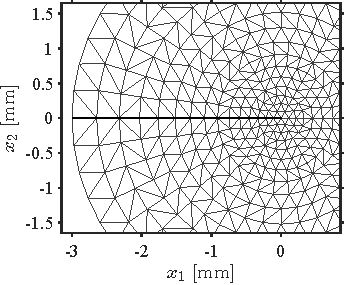
\includegraphics[width=\linewidth]{figures/mesh_levels/tip_mesh_H2.pdf}
    \caption{$4h_0$}
    \label{fig:mesh-level-H2}
  \end{subfigure}
  \hfill
  \begin{subfigure}[t]{0.315\linewidth}
    \centering
    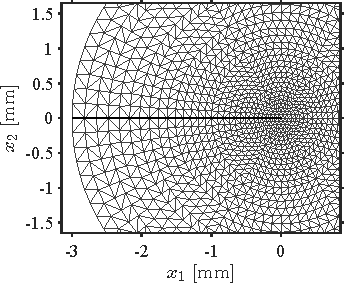
\includegraphics[width=\linewidth]{figures/mesh_levels/tip_mesh_H1.pdf}
    \caption{$2h_0$}
    \label{fig:mesh-level-H1}
  \end{subfigure}
  \hfill
  \begin{subfigure}[t]{0.315\linewidth}
    \centering
    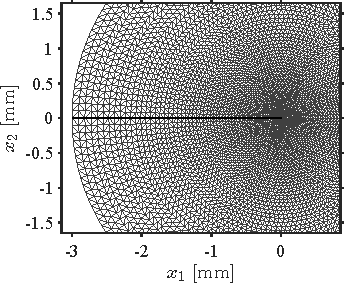
\includegraphics[width=\linewidth]{figures/mesh_levels/tip_mesh_H0.pdf}
    \caption{$h_0$}
    \label{fig:mesh-level-H0}
  \end{subfigure}

  \caption{Structured near-tip mesh hierarchy at a common core radius
  $r_c=3$ mm and identical spatial limits; $h_0=0.027012$ mm denotes
  the finest tip size. The $4h_0$ mesh is shown for geometric illustration
  only: unlike $2h_0$ and $h_0$, it does not meet the native
  COD-sampling requirement.}
  \label{fig:mesh-levels}
\end{figure}

\subsection{Interaction/domain integral}
Let $q$ be a radial domain weight and let $m$ identify an auxiliary
opening or sliding mode. Indices $i,j$ refer to the two tip-local
coordinates and repeated indices are summed; $\delta_{1j}$ is the
Kronecker delta. For the actual field
$(\bm\sigma,\bm\varepsilon,\bm u)$, the interaction integral is
\begin{equation}
 I^{(m)}=\int_{\Omega_k}
 \left[-(\bm\sigma^{(m)}\!:\bm\varepsilon)\delta_{1j}
 +\sigma_{ij}u^{(m)}_{i,1}
 +\sigma^{(m)}_{ij}u_{i,1}\right]q_{,j}\,\dd\Omega,
 \qquad i,j\in\{1,2\}.\label{eq:interaction}
\end{equation}
Actual gradients use the T6 displacement field. Analytical near-tip
auxiliary stresses and centered finite-difference derivatives of auxiliary
displacements are used, with the recorded derivative step
$h=\max(10^{-7}\ \mathrm m,10^{-5}r)$. A radial nodal weight is one for
$r\leq r_i$, decreases linearly to zero at $r_o$, and is zero outside.
Its T6 interpolant supplies the FE-consistent gradient in
Eq.~\eqref{eq:interaction}. Integration uses the 16-point triangular rule.
For auxiliary amplitude $K_{\mathrm{aux}}=1$ and plane strain,
\begin{equation}
 K_m=\frac{E'}{2K_{\mathrm{aux}}}I^{(m)},\qquad
 E'=\frac{E}{1-\nu^2},\qquad m\in\{I,II\}.\label{eq:normalization}
\end{equation}
Here $\dd\Omega$ is the area measure, a comma denotes differentiation,
and the colon denotes tensor contraction. The domain weight $q$ is distinct
from the mode-mixity ratio $q_K$. The normalization preserves the signed local-mode convention.
% TODO: verified interaction-integral and quadrature references.

\subsection{Independent COD postprocessing}
Native upper/lower T6 face nodes are paired in the last-segment frame.
If $[\![u_i]\!]$ denotes the upper-minus-lower displacement jump behind
the tip at distance $r$, the apparent COD SIFs are
\begin{equation}
 \begin{bmatrix}K_I^{\mathrm{app}}(r)\\K_{II}^{\mathrm{app}}(r)\end{bmatrix}
 =\frac{\mu}{\kappa+1}\sqrt{\frac{2\pi}{r}}
 \begin{bmatrix}{[\![u_2]\!]}\\{[\![u_1]\!]}\end{bmatrix},
 \qquad \kappa=3-4\nu.\label{eq:cod}
\end{equation}
Linear and quadratic fits in $r/\Delta a$ extrapolate these quantities to
$r=0$. The four fitting windows are $[0.04,0.20]$, $[0.04,0.30]$,
$[0.08,0.30]$, and $[0.12,0.30]$ times $\Delta a$, with 38, 55, 44,
and 34 native samples. COD verifies a second extraction route from the
\emph{same} elastic field. The production direction always uses the EDI
SIFs; window/order scatter is not a statistical uncertainty interval.

\subsection{Solver and evidence checks}
The unclamped symmetric stiffness is reduced to free degrees of freedom,
symmetrized within the audited formulation, and reordered by a symmetric
approximate minimum-degree permutation. Symmetric Gauss--Seidel preconditioning is used with the preconditioned
conjugate-gradient method (PCG). The
reported-residual tolerance is $10^{-10}$, the iteration limit is 5000,
and the independently computed true-relative-residual gate is
$5\times10^{-10}$. Constrained degrees of freedom remain exactly zero.
For the finer fixed-geometry sensitivity meshes only, MATLAB PCG can report
finite-precision stagnation immediately above the stated tolerance. In that
case one Krylov restart from the returned iterate is permitted, using the
same matrix, right-hand side, SGS factors, tolerance, and iteration limit.
The final PCG and independently recomputed residual gates are unchanged;
a restart therefore resets the recurrence but does not relax acceptance.
Only an accepted elastic field is checkpointed, before SIF/COD/MTS
postprocessing.

Prescribed nodal pure-I, pure-II, and tiny-mixed $(K_I,K_{II})=(1,10^{-4})$
fields test modal recovery and leakage on each qualified mesh. Recovery
and tiny-mixed relative-error gates are $2\times10^{-4}$; the pure-mode
cross-leakage and superposition gates are $10^{-10}$. On the reference meshes, the observed maximum
tiny-mixed relative error is $\SyntheticRelativeError$. These controls
qualify extraction capability and topology rather than the global physical
finite-element error.

The reference history contains accepted physical states through $P_{23}$.
Its continuation $P_{24}$ satisfies geometric and prescribed-field checks
but has no accepted physical solution. For the accepted $P_2$--$P_{23}$
fields, the largest true residual is approximately $\MaxTrueResidual$,
with 2442--3011 PCG iterations. Figure~\ref{fig:quality} collects these
acceptance diagnostics; the saved full-precision records support independent
verification of the reported trajectory and extraction quantities.

\subsection{Crack-increment refinement family}
The finite-step recurrence is assessed with three independently propagated
paths using
\[
 \Delta a\in\{4,2,1\}\ \mathrm{mm}.
\]
All three use the same dimensionless coarse numerical family rather than
the production $h_0$ family. The structured core uses scale factor 2, so that
\begin{equation}
 \frac{h_{\rm tip}}{\Delta a}
 =2(0.00675308135),\qquad
 \frac{r_i}{\Delta a}=0.10,\qquad
 \frac{r_o}{\Delta a}=0.65,\qquad
 \frac{r_c}{\Delta a}=0.75.
 \label{eq:increment-family}
\end{equation}
The exterior uses the M1 dimensionless controls
\[
 \frac{h_{\rm far}}{\Delta a}=1.25,\qquad
 \frac{L_{\rm tr}}{\Delta a}=1.00,
\]
with far-field grading slope 0.15 and boundary-metric growth 0.35.
Therefore halving $\Delta a$ halves the absolute core, EDI, transition,
and exterior length scales while retaining the same numerical family.
This is a refinement study of the complete fixed-increment algorithm in
dimensionless form; it is not an experiment in which $\Delta a$ alone is
changed while an absolute mesh is held fixed.

The accepted Stage-I initiation point and frozen frame are identical for all
three levels. The reserved first-segment length is changed only for Stage II,
$P_1$ is rebuilt and solved independently, and every later vertex is
generated from that path's own SIF/MTS history. Each trajectory is continued
to a common total crack length of 92 mm. Pairwise geometric and direction
differences are evaluated only at exact common crack lengths, using the
4-mm grid as the common set; no path interpolation is used for those
comparisons. The location of local symmetry is reported separately by
linear interpolation between the two solved states that bracket
$q_K=K_{II}/K_I=0$ and is therefore used only as a sub-increment diagnostic.

\subsection{Centered-hole symmetric control}
A separate control problem tests the directional recurrence under exact
reflection symmetry. The full plate dimensions and hole radius are unchanged,
but the circular hole is centered at $(0.150,0)$ m. The crack starts from the
rightmost point of the hole,
\[
 P_0=(0.180,0)\ \mathrm m,
 \qquad
 P_1=(0.184,0)\ \mathrm m,
\]
with the same increment $\Delta a=4$ mm. The straight configuration is
therefore a nominally pure mode-I path. To test its local directional
stability rather than merely verify $K_{II}=0$ at one geometry, five
two-segment probes are prescribed,
\[
 \theta_2\in\{-0.10^\circ,-0.05^\circ,0,
                 +0.05^\circ,+0.10^\circ\},
\]
and each probe is rebuilt and solved independently with the same paired-core,
EDI, solver, and MTS machinery used for the asymmetric calculation. The
resulting one-step map is
\begin{equation}
 F(\theta_2)=\theta_3
 =\theta_2+
 \alpha_{\rm MTS}\!\left(K_I(\theta_2),K_{II}(\theta_2)\right).
 \label{eq:symmetric-map}
\end{equation}

At the straight state,
\[
 K_I(0)=0.42541\ \mathrm{MPa}\sqrt{\mathrm m},
 \qquad
 \frac{K_{II}(0)}{K_I(0)}=6.22\times10^{-9},
\]
and the predicted next direction is
$F(0)=-7.13\times10^{-7}$ degrees, numerically indistinguishable from the
symmetry line at the scale relevant here. The perturbed probes give the
map summarized in Table~\ref{tab:symmetric-stability}.

\begin{table}[tbp]
\centering
\small
\caption{One-step directional map for the centered-hole symmetric control.
Each row is an independently rebuilt and solved two-segment geometry.}
\label{tab:symmetric-stability}
\begin{tabular}{rr}
\toprule
$\theta_2$ [deg] & $F(\theta_2)=\theta_3$ [deg]\\
\midrule
$-0.10$ & $+0.011415$\\
$-0.05$ & $+0.005708$\\
$0$     & $-7.13\times10^{-7}$\\
$+0.05$ & $-0.005708$\\
$+0.10$ & $-0.011415$\\
\bottomrule
\end{tabular}
\end{table}

The recovered opening-mode intensity is even with respect to the imposed
perturbation, whereas $K_{II}/K_I$ and $F(\theta_2)$ are antisymmetric to
within numerical mismatches of order $10^{-9}$. The two symmetric
finite-difference estimates are
\[
 \frac{F(+0.05^\circ)-F(-0.05^\circ)}{0.10^\circ}
 =-0.11416,
 \qquad
 \frac{F(+0.10^\circ)-F(-0.10^\circ)}{0.20^\circ}
 =-0.11415,
\]
and a least-squares fit constrained through the origin gives
\begin{equation}
 F'(0)=-0.11415.
 \label{eq:symmetric-multiplier}
\end{equation}
Because $|F'(0)|<1$, the straight symmetric path is a locally attracting
fixed path for this one-step discrete recurrence. The negative multiplier
means that a small angular perturbation changes sign after one update while
its magnitude is reduced by almost an order of magnitude. This is a local stability statement for the chosen 4-mm recurrence, not a
proof of global path stability. Crack-increment dependence is assessed
independently by the three-level refinement family described above.

\section{Crack-trajectory results}
\label{sec:results}
\subsection{Accepted path and direction history}
The accepted first-tip SIFs at the stated unit traction are
$K_I^{(1)}=0.36648$ and
$K_{II}^{(1)}=4.1983\times10^{-6}$ MPa$\sqrt{\mathrm m}$,
giving $\Delta\theta_2=\theta_2=-0.0013127^\circ$.
The subsequent accepted elastic states are $P_2$ through $P_{23}$.

Figure~\ref{fig:trajectory} distinguishes the accepted $P_0$--$P_{23}$
polyline from the dashed, qualified but unsolved $P_{23}$--$P_{24}$
extension. The accepted crack length is 92 mm. The last tip and its
horizontal clearance from the right boundary are
\begin{equation}
 P_{23}=(\LastXMM,\LastYMM)\ \mathrm{mm},\qquad
 2A-x_{23}=\LastLigamentMM\ \mathrm{mm}.
\end{equation}
Directions vary gradually, although the
finite-increment representation is piecewise linear rather than a
continuously smooth curve.

The absolute direction becomes increasingly negative up to
$\theta_{22}=\MinimumTheta^\circ$, then rotates toward a less negative
inclination at $P_{23}$ (Fig.~\ref{fig:intensities}). A positive late turn
does not imply an upward-moving tip: the accepted segments remain
negatively inclined and their global $y$ coordinates continue to decrease.

% Figure environment maintained inline in main.tex; graphics remain separate PDFs.
\begin{figure}[tbp]
  \centering
  \begin{subfigure}[t]{0.94\linewidth}
    \centering
    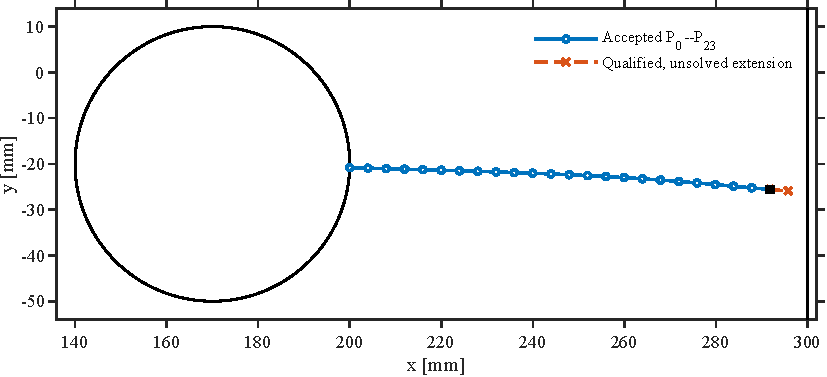
\includegraphics[width=\linewidth]{figures/trajectory/overview.pdf}
    \caption{Hole and accepted trajectory through $P_{23}$, with the
    qualified but physically unsolved $P_{23}$--$P_{24}$ extension.}
    \label{fig:trajectory-overview}
  \end{subfigure}

  \medskip

  \begin{subfigure}[t]{0.94\linewidth}
    \centering
    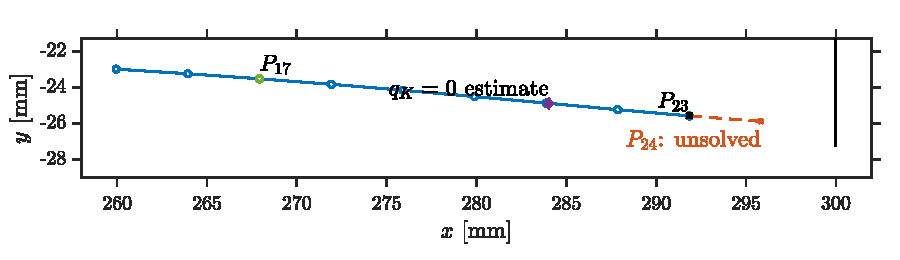
\includegraphics[width=\linewidth]{figures/trajectory/late_detail.pdf}
    \caption{Late-path detail with equal spatial scales. The markers identify
    $P_{17}$, the linearly interpolated $K_{II}/K_I=0$ location, $P_{23}$,
    and the qualified unsolved point $P_{24}$.}
    \label{fig:trajectory-late}
  \end{subfigure}

  \caption{Hole-initiated trajectory and late detail. Both spatial panels
  use equal $x$ and $y$ scales within the panel. The circle gives geometric
  context; the numerical hole is polygonally discretized. Solid segments are
  accepted geometry through $P_{23}$. The dashed extension is qualified
  geometry only and has no accepted physical SIFs. The diamond is a linear
  interpolation marker, not a solved tip.}
  \label{fig:trajectory}
\end{figure}


\subsection{Mode intensities and the positive maximum}
Figure~\ref{fig:intensities} shows monotonically increasing $K_I$, from
0.36648 at $P_1$ to 1.2444 at $P_{23}$. The initially very small positive
$K_{II}$ grows to its positive maximum at $P_{17}$, where $a=68$ mm,
$K_{II}=0.0025484$, and $\qmix=K_{II}/K_I=0.0032389$.
The positive mode-mixity maximum occurs at the same state. It is not the
maximum \emph{absolute} mode-II intensity: the negative mode-II magnitude
at the last accepted tip is larger.

From $P_{17}$ through $P_{21}$, $K_{II}$ remains positive but decreases.
Accordingly the negative incremental MTS turn becomes smaller in
magnitude (Fig.~\ref{fig:late}). This change in turning response accompanies
an increasing opening-mode intensity, not unloading.

% Figure environment maintained inline in main.tex; graphics remain separate PDFs.
\begin{figure}[tbp]
  \centering
  \begin{subfigure}[t]{0.82\linewidth}
    \centering
    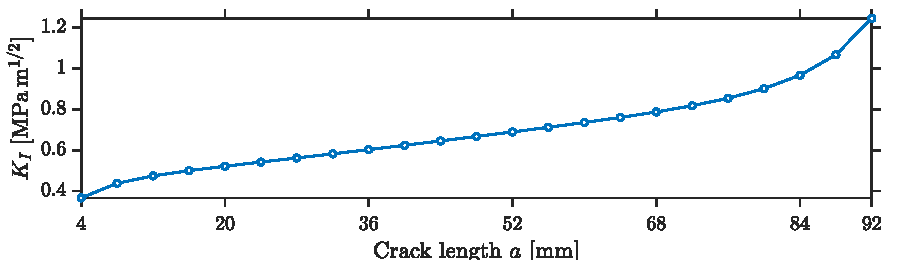
\includegraphics[width=\linewidth]{figures/intensities/KI.pdf}
    \caption{Opening-mode factor $K_I$.}
    \label{fig:intensities-KI}
  \end{subfigure}

  \smallskip

  \begin{subfigure}[t]{0.82\linewidth}
    \centering
    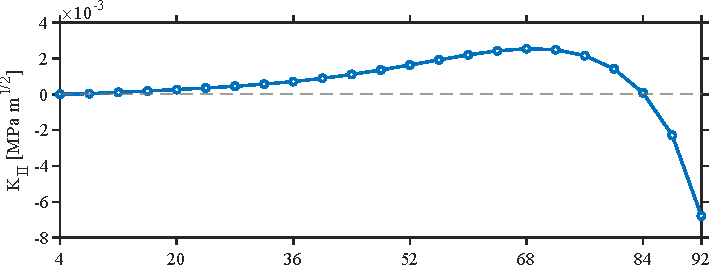
\includegraphics[width=\linewidth]{figures/intensities/KII.pdf}
    \caption{Sliding-mode factor $K_{II}$.}
    \label{fig:intensities-KII}
  \end{subfigure}

  \smallskip

  \begin{subfigure}[t]{0.82\linewidth}
    \centering
    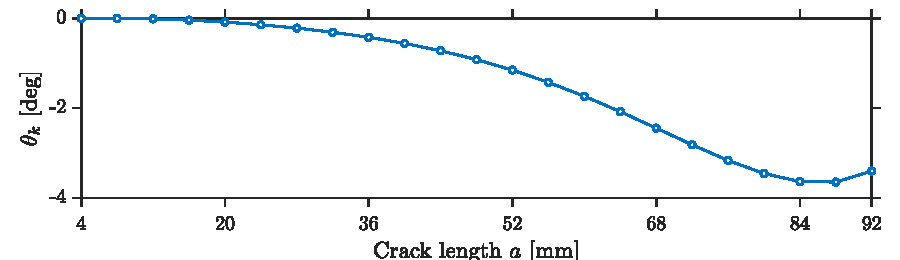
\includegraphics[width=\linewidth]{figures/intensities/theta.pdf}
    \caption{Absolute direction $\theta_k$.}
    \label{fig:intensities-theta}
  \end{subfigure}

  \caption{Accepted intensities and absolute direction in the frozen
  initiation frame. Intensities correspond to unit remote traction. The
  direction minimum occurs at $P_{22}$; positive turning there produces the
  less negative $P_{23}$ direction. No physical curve includes $P_{24}$.}
  \label{fig:intensities}
\end{figure}


\subsection{Local-symmetry crossing and late turning reversal}
At $P_{21}$ ($a=84$ mm), $\qmix=+8.134267\times10^{-5}$; at $P_{22}$
($a=88$ mm), $\qmix=-0.0021416$. The sign change is therefore bracketed
by two solved states. For visualization only, linear interpolation gives
\begin{equation}
 a_{\mathrm{LS}}=a_{21}
 -\frac{\qmix^{(21)}}{\qmix^{(22)}-\qmix^{(21)}}(a_{22}-a_{21})
 \simeq\LSLengthMM\ \mathrm{mm}.\label{eq:zeroestimate}
\end{equation}
This estimate is not an independently solved local-symmetry state and does
not quantify interpolation or increment-size error.

Mode II is negative at $P_{22}$ and $P_{23}$, so the next turning increments
are positive. The last accepted state has $K_I=1.2444$,
$K_{II}=-0.0067803$, and $\qmix=-0.0054488$. It predicts
$\Delta\theta_{24}=0.62435^\circ$ and
$\theta_{24}=-2.7762^\circ$. The latter defines the next qualified
geometry, not a physical solution at $P_{24}$.

\begin{table}[tbp]\centering\small\setlength{\tabcolsep}{3.5pt}
\caption{Characteristic accepted states. SIFs have units MPa$\sqrt{\mathrm m}$;
angles are in degrees. The interpolated row contains only a graphical
zero estimate, not a solved stress field or crack direction.}
\begin{tabular}{lrrrrrr}\toprule
State & $a$ [mm] & $K_I$ & $K_{II}$ & $K_{II}/K_I$ & $\theta_k$ & $\Delta\theta_{k+1}$\\\midrule
\CharacteristicRows
Interpolated & \LSLengthMM & --- & --- & $0$ & --- & ---\\
\bottomrule\end{tabular}\label{tab:states}
\end{table}

% Figure environment maintained inline in main.tex; graphics remain separate PDFs.
\begin{figure}[tbp]
  \centering
  \begin{subfigure}[t]{0.82\linewidth}
    \centering
    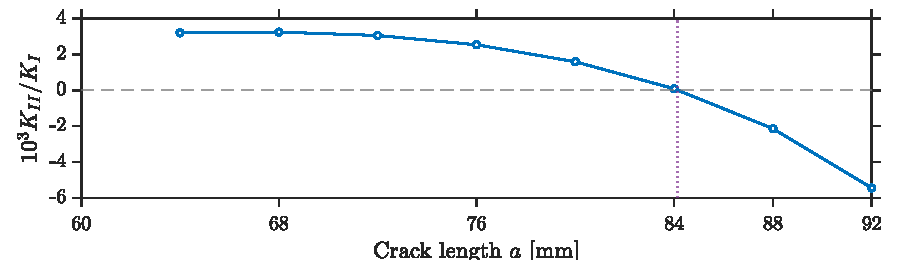
\includegraphics[width=\linewidth]{figures/late/mode_mixity.pdf}
    \caption{Late mode-mixity history.}
    \label{fig:late-mixity}
  \end{subfigure}

  \smallskip

  \begin{subfigure}[t]{0.82\linewidth}
    \centering
    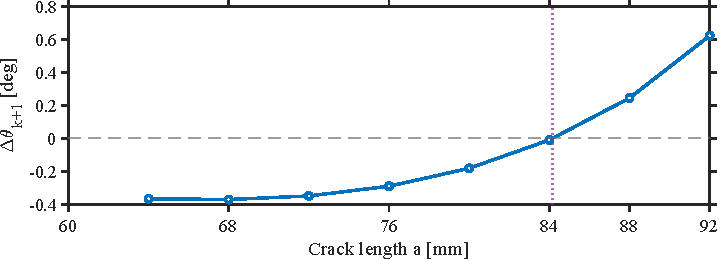
\includegraphics[width=\linewidth]{figures/late/turn.pdf}
    \caption{Incremental MTS turn.}
    \label{fig:late-turn}
  \end{subfigure}

  \caption{Mode-mixity sign reversal and opposite-signed MTS turning.
  Each marker is an accepted current-tip state; its turn predicts the next
  segment. The vertical dotted line is the interpolated $K_{II}/K_I=0$
  location. The positive turn reported at $a=92$ mm belongs to the $P_{23}$
  solution and predicts the unsolved next geometry.}
  \label{fig:late}
\end{figure}


\subsection{COD comparison and extraction sensitivity}
All eight stored COD fit definitions retain positive mode mixity at $P_{21}$
and negative mode mixity at $P_{22}$, corroborating the bracketed sign change
without making COD the direction selector. Differences remain nonzero and
depend on the fitting definition (Fig.~\ref{fig:cod}). Over all 176 fits,
the largest absolute COD--EDI turning difference is $\MaxCODError^\circ$,
at $P_{23}$ for a linear fit over $[0.12,0.30]\Delta a$.
The quadratic-fit turns at $P_{23}$ range from $\CODQuadMin^\circ$ to
$\CODQuadMax^\circ$, compared with the EDI value $0.62435^\circ$.

Near local symmetry, relative differences can be large despite small
absolute errors. At $P_{21}$ the same rear-window linear fit gives mode
mixity about $\CODNearZeroPercent$\% above EDI, while its turning-angle
difference is only $\CODNearZeroTurnDiff^\circ$. Thus visual overlap of
full-history curves is not sufficient to establish extraction accuracy.
The late fitting sensitivity is a postprocessing limitation to investigate,
not an error bar on the physical path. Both routes also share any error in
the underlying elastic solution.

% Figure environment maintained inline in main.tex; graphics remain separate PDFs.
\begin{figure}[tbp]
  \centering
  \begin{subfigure}[t]{0.485\linewidth}
    \centering
    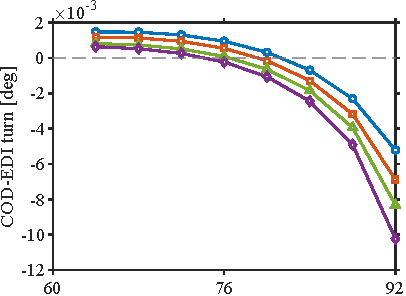
\includegraphics[width=\linewidth]{figures/cod/turn_linear.pdf}
    \caption{Turning-angle differences for linear COD fits.}
    \label{fig:cod-turn-linear}
  \end{subfigure}
  \hfill
  \begin{subfigure}[t]{0.485\linewidth}
    \centering
    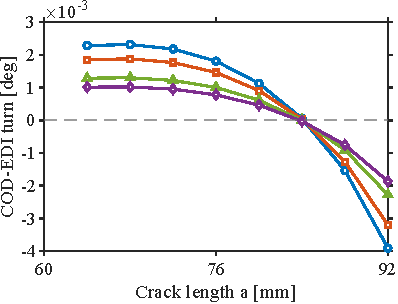
\includegraphics[width=\linewidth]{figures/cod/turn_quadratic.pdf}
    \caption{Turning-angle differences for quadratic COD fits.}
    \label{fig:cod-turn-quadratic}
  \end{subfigure}

  \medskip

  \begin{subfigure}[t]{0.485\linewidth}
    \centering
    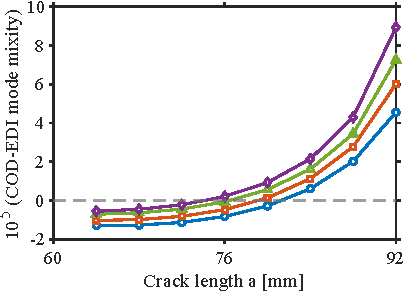
\includegraphics[width=\linewidth]{figures/cod/mixity_linear.pdf}
    \caption{Mode-mixity differences for linear COD fits.}
    \label{fig:cod-mixity-linear}
  \end{subfigure}
  \hfill
  \begin{subfigure}[t]{0.485\linewidth}
    \centering
    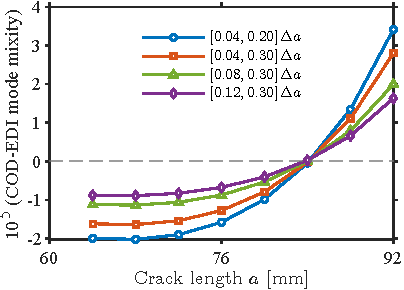
\includegraphics[width=\linewidth]{figures/cod/mixity_quadratic.pdf}
    \caption{Mode-mixity differences for quadratic COD fits.}
    \label{fig:cod-mixity-quadratic}
  \end{subfigure}

  \caption{Late-path extraction differences for all four native COD windows
  and both polynomial degrees. Window bounds are multiples of $\Delta a$.
  Zero is equality with EDI, not a known exact solution. The upper panels
  show differences in the MTS turns computed from the two sets of SIFs;
  the lower panels show differences in mode mixity. The largest observed
  difference occurs at the last accepted tip; individual difference curves
  need not vary monotonically.}
  \label{fig:cod}
\end{figure}


\subsection{Sensitivity to structured-tip resolution}
For comparisons at matched crack lengths, $\delta x$ and $\delta y$ denote
coordinate differences between the compared and reference paths,
$\delta r=(\delta x^2+\delta y^2)^{1/2}$ is their separation, and
$\delta\theta$ is the difference of absolute directions in the frozen
frame. The symbol $\Delta\theta_{k+1}$ remains reserved for a local MTS
turn. Differences in mode mixity and interpolated crossing length are
denoted by $\delta q_K$ and $\delta a_{\mathrm{LS}}$, respectively.

The fixed-geometry three-level comparison changes the structured-tip
resolution with the requested exterior sizing law held at its reference
value. At $P_{17}$, halving the production tip size from
$0.027012$ to $0.013506$ mm changes $K_I$ by $0.00134\%$,
$K_{II}/K_I$ by $1.05\times10^{-6}$ in absolute value, and the MTS turn by
only $-1.20\times10^{-4}$ degrees. Thus the positive mode-mixity maximum is
stable under this structured-tip refinement at fixed requested exterior sizing.

The more discriminating comparison is the $P_{21}$--$P_{22}$ bracket, where
$K_{II}$ changes sign. Table~\ref{tab:tipmesh} shows three physically
qualified levels spanning a factor of four in $h_{\mathrm{tip}}$. Every
level keeps $K_{II}/K_I>0$ at $P_{21}$ and $K_{II}/K_I<0$ at $P_{22}$, so
the local-symmetry bracket and the associated reversal of MTS turning sense
are unchanged.

\begin{table}[tbp]
\centering
\small
\setlength{\tabcolsep}{2.8pt}
\caption{Fixed-geometry sensitivity to structured-tip resolution. The crack
geometries at $P_{21}$ and $P_{22}$, material, loading, EDI radii, far-field
cap, transition length, and MTS formulation are unchanged; the structured
tip scale changes while $\eta_e=1$ fixes the requested
exterior sizing law. Exterior connectivity need not be identical. The final column is an interpolation between solved values, not a solved
crack state; its extra digits resolve numerical mesh-comparison shifts only.}
\label{tab:tipmesh}
\begin{tabular}{lrrrrrr}
\toprule
Resolution & $h_{\rm tip}$ [mm] &
$q_K(P_{21})$ & $\Delta\theta_{22}$ [deg] &
$q_K(P_{22})$ & $\Delta\theta_{23}$ [deg] &
$a_{\rm LS}$ [mm]\\
\midrule
$2h_0$ & 0.054025 & $+7.7957\times10^{-5}$ & $-0.008933$ &
$-2.1451\times10^{-3}$ & $+0.245805$ & 84.14027\\
$h_0$ & 0.027012 & $+8.1343\times10^{-5}$ & $-0.009321$ &
$-2.1416\times10^{-3}$ & $+0.245406$ & 84.14637\\
$h_0/2$ & 0.013506 & $+8.3031\times10^{-5}$ & $-0.009515$ &
$-2.1399\times10^{-3}$ & $+0.245207$ & 84.14941\\
\bottomrule
\end{tabular}
\end{table}

The interpolated crossing moves from $84.14027$ mm at $2h_0$ to
$84.14637$ mm at $h_0$ and $84.14941$ mm at $h_0/2$. The successive
changes, $6.10~\mu\mathrm{m}$ and $3.04~\mu\mathrm{m}$, are tiny relative
to the 4-mm crack increment. Taken only as a three-level diagnostic, their
ratio corresponds to an observed order of approximately $1.00$ for this
interpolated quantity. The exterior is remeshed to conform to each core and the crossing
is inferred between states separated by one full crack increment. This
three-level regularity is therefore not treated as a formal convergence
order or as micrometer-scale physical accuracy.

The independent $2h_0$ trajectory tests whether these small fixed-geometry
differences accumulate along the path. Figure~
\ref{fig:tip-resolution-sensitivity} uses the same four-panel comparison as
the exterior-mesh study. The trajectories are visually indistinguishable
at specimen scale [Fig.~\ref{fig:tipres-trajectory}]. Over the full accepted
history, the maximum vertical-coordinate difference is
$0.12760~\mu\mathrm{m}$ and the maximum Euclidean separation of
corresponding tips is $0.12800~\mu\mathrm{m}$, both at $P_{23}$. The
maximum absolute direction difference is $0.24539$ millidegrees at
$P_{22}$ [Figs.~\ref{fig:tipres-dy} and \ref{fig:tipres-dtheta}].

The mechanical history is equally stable. Both mesh families place the
positive maximum of $K_{II}/K_I$ at $P_{17}$ and retain positive mode
mixity at $P_{21}$ and negative mode mixity at $P_{22}$
[Fig.~\ref{fig:tipres-q}]. The maximum absolute difference in
$K_{II}/K_I$ is $2.65\times10^{-7}$. Linear interpolation of the two
independently propagated $P_{21}$--$P_{22}$ brackets gives
$a_{\mathrm{LS}}=84.14637$ mm for $h_0$ and
$84.146276$ mm for $2h_0$, a difference of
$-0.000094$ mm ($-0.094~\mu\mathrm{m}$). As above, this is only a
sub-increment sensitivity diagnostic, not a micrometer-accurate physical
location of local symmetry.

The fixed-geometry and independent-path results therefore show that the
reported characteristic events are insensitive to the tested structured-tip
resolution changes with the requested exterior sizing law fixed. This
parameter isolation does not imply identical exterior connectivity or bound
every discretization error.

% Figure environment maintained inline in main.tex; graphics remain separate PDFs.
\begin{figure}[tbp]
  \centering

  \begin{subfigure}[t]{0.94\linewidth}
    \centering
    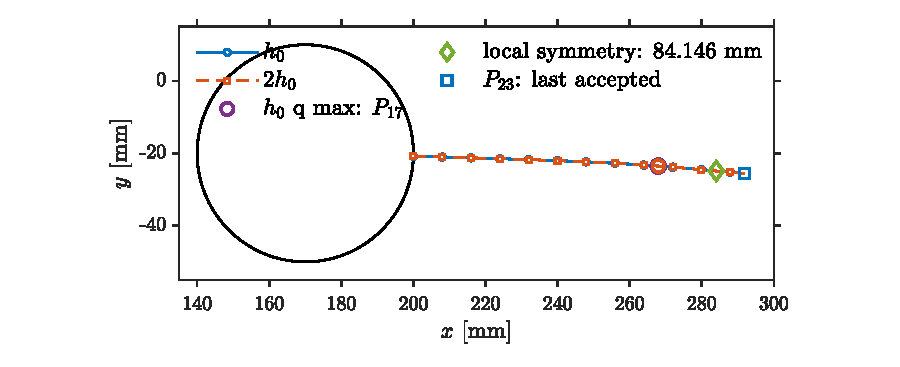
\includegraphics[width=\linewidth]{figures/tip_resolution_sensitivity/trajectory.pdf}
    \caption{Independently propagated trajectories for the production
    $h_0$ mesh family and the coarser $2h_0$ structured core at fixed requested exterior sizing. The two
    paths are visually indistinguishable at the scale of the specimen.}
    \label{fig:tipres-trajectory}
  \end{subfigure}

  \medskip

  \begin{subfigure}[t]{0.315\linewidth}
    \centering
    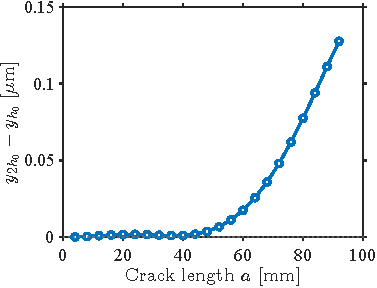
\includegraphics[width=\linewidth]{figures/tip_resolution_sensitivity/vertical_deviation.pdf}
    \caption{Accumulated vertical tip-coordinate difference,
    $y_{2h_0}-y_{h_0}$.}
    \label{fig:tipres-dy}
  \end{subfigure}
  \hfill
  \begin{subfigure}[t]{0.315\linewidth}
    \centering
    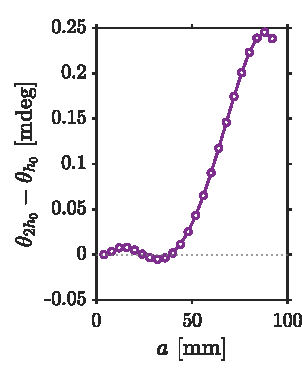
\includegraphics[width=\linewidth]{figures/tip_resolution_sensitivity/direction_deviation.pdf}
    \caption{Difference in the absolute crack direction in the frozen initiation frame,
    $\theta_{2h_0}-\theta_{h_0}$.}
    \label{fig:tipres-dtheta}
  \end{subfigure}
  \hfill
  \begin{subfigure}[t]{0.315\linewidth}
    \centering
    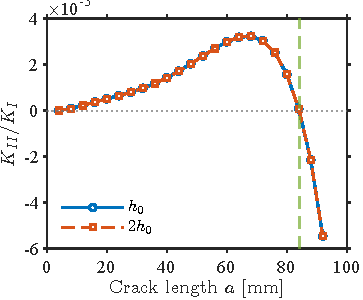
\includegraphics[width=\linewidth]{figures/tip_resolution_sensitivity/mode_mixity.pdf}
    \caption{Mode-mixity ratio $K_{II}/K_I$ along the two independently
    propagated trajectories.}
    \label{fig:tipres-q}
  \end{subfigure}

  \caption{Sensitivity of the incremental LEFM trajectory to
  structured-tip resolution. The $2h_0$ calculation doubles the production
  tip size from $h_0=0.027012$ mm to $0.054025$ mm while retaining the
  interaction-domain radii, far-field cap, and transition length.
  $\eta_e=1$ preserves the requested exterior sizing law;
  the conforming exterior connectivity need not be identical. The $2h_0$
  trajectory is propagated independently from a recomputed $P_1$ field
  rather than from reference vertices. The local-symmetry marker is the
  linearly interpolated reference crossing, not an independently solved state.}
  \label{fig:tip-resolution-sensitivity}
\end{figure}

\subsection{Sensitivity to exterior-mesh density}
The fixed-geometry M1 checks establish that the coarser exterior mesh does
not materially perturb the extracted current-tip quantities when the crack
polyline is held fixed. To test accumulated trajectory sensitivity, however,
the M1 path was regenerated independently rather than evaluated on the
reference vertices. The prescribed first segment $P_0P_1$ is common to both
calculations, but the $P_1$ elastic problem is resolved on M1, its own
$K_I^{(1)}$ and $K_{II}^{(1)}$ determine $\theta_2$, and every subsequent
vertex follows recursively from the preceding M1 solution. Thus no
reference-path vertex after $P_1$ is imposed.

Figure~\ref{fig:m1-mesh-sensitivity} compares the two complete accepted
histories through $P_{23}$. At specimen scale the trajectories are visually
indistinguishable [Fig.~\ref{fig:m1mesh-trajectory}]. The accumulated
difference is resolved by plotting the coordinate and direction differences
directly. Over all common accepted states, the maximum vertical-coordinate
difference is $0.06734~\mu\mathrm{m}$, the maximum Euclidean separation of
corresponding tips is $0.06742~\mu\mathrm{m}$, and the maximum absolute direction
difference is $0.07304$ millidegrees, or $7.30\times10^{-5}$ degrees
[Figs.~\ref{fig:m1mesh-dy} and \ref{fig:m1mesh-dtheta}].

The mechanical history is equally stable. Both calculations place the
positive maximum of $K_{II}/K_I$ at $P_{17}$ ($a=68$ mm), and both retain
positive mode mixity at $P_{21}$ and negative mode mixity at $P_{22}$
[Fig.~\ref{fig:m1mesh-q}]. The maximum absolute difference in
$K_{II}/K_I$ over the accepted histories is $2.89\times10^{-7}$. Linear
interpolation of the two respective $P_{21}$--$P_{22}$ brackets gives
$a_{\mathrm{LS}}=84.14637$ mm for the reference trajectory and
$84.146$ mm for M1, a difference of $0.000322$ mm
($0.322~\mu\mathrm{m}$). This sub-increment difference is reported only as a
sensitivity diagnostic; neither interpolated value has physical precision
at the micrometer scale.

The result therefore supports robustness of the reported mode-mixity
maximum, sign reversal, and late turning response with respect to a
substantial coarsening of the \emph{exterior} mesh. It is deliberately
narrower than a general mesh-independence claim because the paired tip core
and interaction-domain radii are held fixed. Local tip-resolution sensitivity
is examined separately above, whereas interaction-domain-radius sensitivity
remains unresolved.

% Figure environment maintained inline in main.tex; graphics remain separate PDFs.
\begin{figure}[tbp]
  \centering

  \begin{subfigure}[t]{0.94\linewidth}
    \centering
    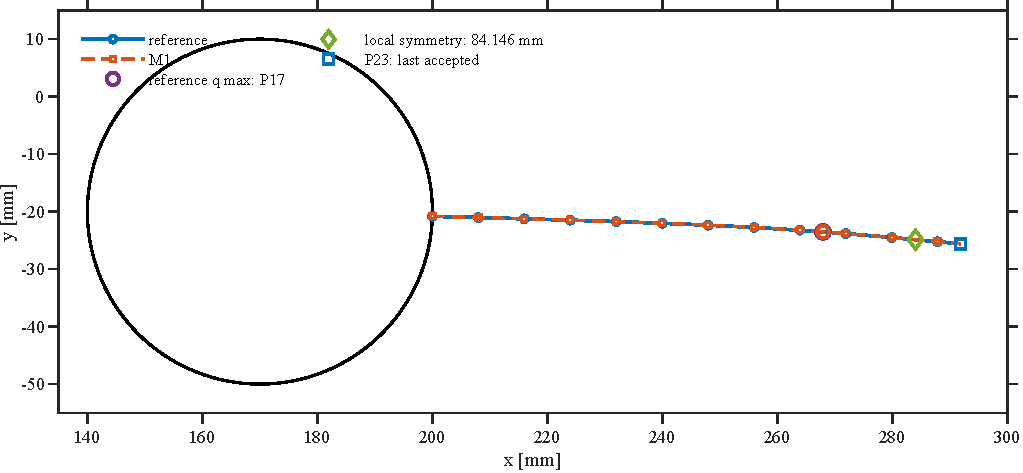
\includegraphics[width=\linewidth]{figures/m1_mesh_sensitivity/trajectory.pdf}
    \caption{Actual crack trajectories obtained with the reference exterior
    mesh and the independently propagated M1 exterior mesh. The two paths
    are visually indistinguishable at the scale of the specimen.}
    \label{fig:m1mesh-trajectory}
  \end{subfigure}

  \medskip

  \begin{subfigure}[t]{0.315\linewidth}
    \centering
    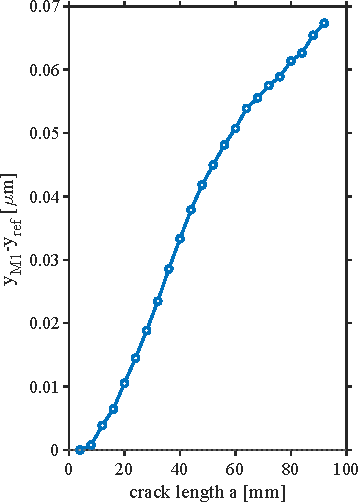
\includegraphics[width=\linewidth]{figures/m1_mesh_sensitivity/vertical_deviation.pdf}
    \caption{Accumulated vertical tip-coordinate difference,
    $y_{\mathrm{M1}}-y_{\mathrm{ref}}$.}
    \label{fig:m1mesh-dy}
  \end{subfigure}
  \hfill
  \begin{subfigure}[t]{0.315\linewidth}
    \centering
    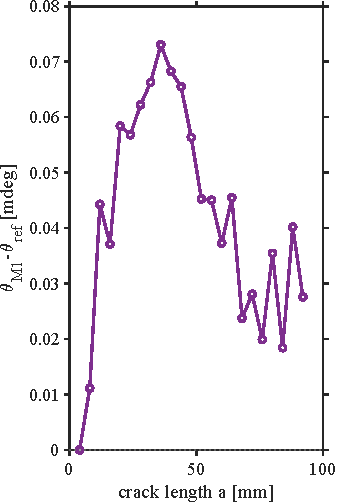
\includegraphics[width=\linewidth]{figures/m1_mesh_sensitivity/direction_deviation.pdf}
    \caption{Difference in the absolute crack direction in the frozen initiation frame,
    $\theta_{\mathrm{M1}}-\theta_{\mathrm{ref}}$.}
    \label{fig:m1mesh-dtheta}
  \end{subfigure}
  \hfill
  \begin{subfigure}[t]{0.315\linewidth}
    \centering
    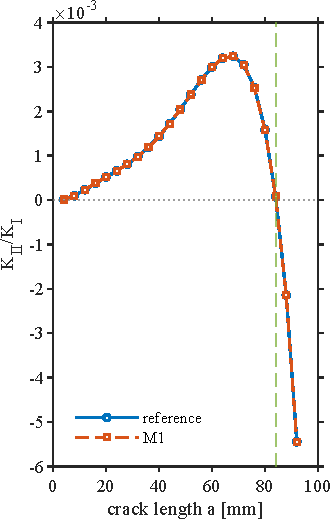
\includegraphics[width=\linewidth]{figures/m1_mesh_sensitivity/mode_mixity.pdf}
    \caption{Mode-mixity ratio $K_{II}/K_I$ along the two independently
    propagated trajectories.}
    \label{fig:m1mesh-q}
  \end{subfigure}

  \caption{Sensitivity of the incremental LEFM trajectory to coarsening of
  the exterior mesh. The M1 calculation retains the audited crack-tip core
  and EDI extraction region but uses a substantially coarser exterior mesh.
  The comparison is based on two independently propagated trajectories:
  the M1 calculation recomputes the $P_1$ SIFs and every subsequent MTS
  update rather than reusing the reference vertices. The local-symmetry
  diamond marks the interpolated reference crossing, not a solved tip.}
  \label{fig:m1-mesh-sensitivity}
\end{figure}

\subsection{Crack-increment sensitivity}
The three-level increment study compares independently generated
$\Delta a=4$, 2, and 1 mm trajectories over the exact common range
4--92 mm. Figure~\ref{fig:increment-sensitivity} shows the three actual
paths together with the successive vertical and directional differences and
the turning density. At specimen scale the trajectories nearly overlap
[Fig.~\ref{fig:inc-trajectory}], whereas the difference panels resolve a
systematic reduction of the accumulated path error when the increment is
halved [Figs.~\ref{fig:inc-dy} and \ref{fig:inc-dtheta}].

% Figure environment maintained inline in main.tex; graphics remain separate PDFs.
\begin{figure}[tbp]
  \centering

  \begin{subfigure}[t]{0.94\linewidth}
    \centering
    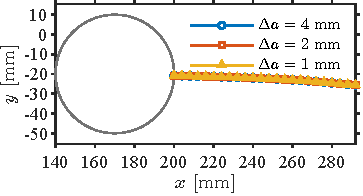
\includegraphics[width=\linewidth]{figures/increment_sensitivity/trajectory.pdf}
    \caption{Independently propagated crack trajectories for
    $\Delta a=4$, 2, and 1 mm, all continued to 92 mm.}
    \label{fig:inc-trajectory}
  \end{subfigure}
  \par\medskip
  \begin{subfigure}[t]{0.315\linewidth}
    \centering
    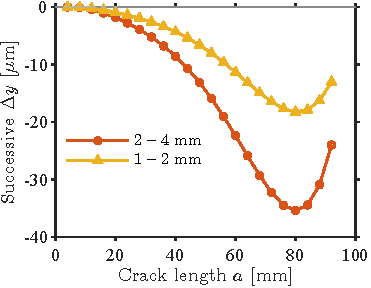
\includegraphics[width=\linewidth]{figures/increment_sensitivity/vertical_deviation.pdf}
    \caption{Successive vertical-coordinate differences,
    $y_{2\,\mathrm{mm}}-y_{4\,\mathrm{mm}}$ and
    $y_{1\,\mathrm{mm}}-y_{2\,\mathrm{mm}}$, evaluated at exact
    common crack lengths.}
    \label{fig:inc-dy}
  \end{subfigure}
  \hfill
  \begin{subfigure}[t]{0.315\linewidth}
    \centering
    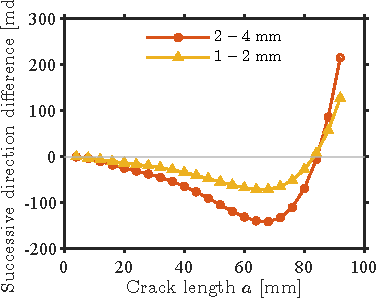
\includegraphics[width=\linewidth]{figures/increment_sensitivity/direction_deviation.pdf}
    \caption{Successive differences in absolute crack direction in the
    frozen initiation frame.}
    \label{fig:inc-dtheta}
  \end{subfigure}
  \hfill
  \begin{subfigure}[t]{0.315\linewidth}
    \centering
    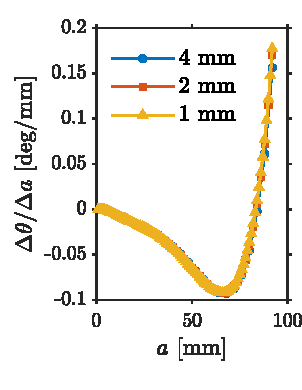
\includegraphics[width=\linewidth]{figures/increment_sensitivity/turn_density.pdf}
    \caption{Turning density $\Delta\theta/\Delta a$ along the three
    independently propagated trajectories.}
    \label{fig:inc-turn-density}
  \end{subfigure}

  \caption{Crack-increment sensitivity of the independently propagated
  LEFM paths. All three calculations use the same dimensionless coarse
  numerical family, with the absolute core, interaction-domain, transition,
  and exterior length scales reduced together with $\Delta a$. The
  trajectory panel shows the actual paths, while the two difference panels
  resolve successive changes at exact common crack lengths. The turning-
  density panel is plotted on each level's native crack-length grid.}
  \label{fig:increment-sensitivity}
\end{figure}

Table~\ref{tab:increment-pairwise} quantifies these successive differences.
Halving the increment from 4 to 2 mm gives a maximum corresponding-tip
separation of $35.472~\mu\mathrm{m}$; halving it again to 1 mm reduces that
maximum to $18.291~\mu\mathrm{m}$. The corresponding maximum
vertical-coordinate differences are $35.418$ and $18.263~\mu\mathrm{m}$.
The maximum absolute direction difference likewise falls from $214.931$ to
$127.391$ millidegrees.

\begin{table}[tbp]
\centering
\small
\setlength{\tabcolsep}{4.0pt}
\caption{Successive differences between independently propagated paths in
the dimensionless crack-increment refinement family. Comparisons use exact
common crack lengths; no path interpolation is used.}
\label{tab:increment-pairwise}
\begin{tabular}{lrrrr}
\toprule
Comparison &
$\max|\delta y|$ [$\mu$m] &
$\max\delta r$ [$\mu$m] &
$\max|\delta\theta|$ [mdeg] &
$\max|\delta q_K|$\\
\midrule
2 mm $-$ 4 mm & 35.4181 & 35.4721 & 214.931 & $2.48578\times10^{-3}$\\
1 mm $-$ 2 mm & 18.2629 & 18.2911 & 127.391 & $1.41618\times10^{-3}$\\
\bottomrule
\end{tabular}
\end{table}

The successive contraction ratios are 1.939 for the maximum tip separation
and 1.687 for the maximum direction difference. If these ratios are
converted only as diagnostics through
$p=\log_2(d_{\Delta a}/d_{\Delta a/2})$, where $d$ denotes the selected successive-difference maximum, they correspond to
$p\simeq0.96$ and $p\simeq0.75$, respectively. Because the trajectory is
generated recursively and the reported quantities are maxima that need not
occur at the same crack length, these values are not treated as formal
Richardson orders. They do, however, show clear contraction of both the
accumulated path and direction differences under successive halving of the
increment.

A more revealing pattern appears in the mode-mixity correction.
Table~\ref{tab:increment-characteristic} lists the positive maximum of
$q_K=K_{II}/K_I$ for each level. The raw maximum decreases almost in direct
proportion to $\Delta a$: from $3.23937\times10^{-3}$ at 4 mm to
$1.61266\times10^{-3}$ at 2 mm and $8.04068\times10^{-4}$ at 1 mm.
In contrast, the normalized quantity $q_{K,\max}/\Delta a$ changes by only
about $0.71\%$ over the entire 4-to-1-mm refinement. The MTS turning density at the same characteristic state is similarly
stable, varying from $-0.092799$ to $-0.092139$ deg/mm. The complete
turning-density histories in Fig.~\ref{fig:inc-turn-density} show that this
agreement is not confined to a single state: refinement primarily resolves
the same smooth variation on progressively finer crack-length grids.

\begin{table}[tbp]
\centering
\small
\setlength{\tabcolsep}{3.6pt}
\caption{Characteristic quantities in the crack-increment refinement
family. The local-symmetry location is obtained by linear interpolation
between the two solved states bracketing $q_K=0$.}
\label{tab:increment-characteristic}
\begin{tabular}{rrrrrr}
\toprule
$\Delta a$ [mm] &
$a(q_{K,\max})$ [mm] &
$q_{K,\max}$ &
$q_{K,\max}/\Delta a$ [mm$^{-1}$] &
$(\Delta\theta/\Delta a)_{q_{\max}}$ [deg/mm] &
$a_{\rm LS}$ [mm]\\
\midrule
4 & 68 & $3.2394\times10^{-3}$ & $8.0984\times10^{-4}$ &
$-0.092799$ & 84.148913\\
2 & 66 & $1.6127\times10^{-3}$ & $8.0633\times10^{-4}$ &
$-0.092398$ & 83.550120\\
1 & 66 & $8.0407\times10^{-4}$ & $8.0407\times10^{-4}$ &
$-0.092139$ & 83.268112\\
\bottomrule
\end{tabular}
\end{table}

This behavior is consistent with
\begin{equation}
 q_K=O(\Delta a),\qquad
 \Delta\theta=O(\Delta a)
 \label{eq:increment-scaling}
\end{equation}
along a smooth limiting trajectory, while $q_K/\Delta a$ and
$\Delta\theta/\Delta a$ remain finite measures of the local corrective
response and turning density. Equation~\eqref{eq:increment-scaling} is an
interpretation of the observed three-level trend, not an independently
proved asymptotic result.

The local-symmetry crossing also contracts systematically. The interpolated
locations are 84.148913, 83.550120, and 83.268112 mm for the 4-, 2-, and
1-mm paths. The successive shifts are therefore $0.59879$ and $0.28201$ mm,
whose ratio is 2.12. Interpreted only as a three-level diagnostic this gives
an apparent order of about 1.09 for the interpolated event location. The
crossing is directly bracketed between the solved 83- and 84-mm states on
the 1-mm path, but it remains an interpolated quantity rather than an
independently solved zero-$K_{II}$ state.

The combined result is stronger than visual path overlap alone. The
trajectory panel establishes the common macroscopic path, while the
successive-difference panels show that the remaining geometric and
directional discrepancies contract under refinement. At the same time, the
raw mode-II correction becomes smaller in proportion to the discrete step. This distinction is important when
interpreting $q_K$: its absolute value along a finite-step MTS path is a
step-dependent corrective quantity, whereas its increment-normalized form
has the more stable continuous-path interpretation.

\section{Discussion}
\label{sec:discussion}
\subsection{Interpretation of late redirection}
The accepted sequence shows reorientation under increasing $K_I$.
The change in turning sign is directly associated with the change in
$K_{II}/K_I$, as required by Eqs.~\eqref{eq:trt}--\eqref{eq:angleupdate}.
The shrinking right-side ligament makes increased free-boundary influence
a consistent physical interpretation. However, the boundary distance and
the accumulated crack geometry change together. A control with a more
distant boundary, or matched fixed-geometry calculations, is needed to
isolate that influence. The result supports a mode-mixity explanation of
the computed redirection; it does not prove that the boundary is its sole
cause.

\subsection{Discretization, increment size, and boundary proximity}
The 4-mm reference trajectory samples a continuously changing boundary-value
problem at discrete geometries, so the finite segment length is part of the
numerical propagation rule. The three-level increment study now provides a
direct measure of this effect. Successive halving from 4 to 2 to 1 mm
reduces the maximum corresponding-tip separation from $35.47$ to
$18.29~\mu\mathrm{m}$ and the maximum direction difference from
$214.93$ to $127.39$ millidegrees. The local-symmetry estimate shifts by
$0.599$ mm and then $0.282$ mm. These contractions support a stable limiting
trajectory, although three levels are insufficient to establish a formal
asymptotic convergence order. The result complements the two-increment
comparison of Fang et al.~\cite{FangEtAl2020}, who observed similar but
smoother crack paths at smaller prescribed increments: here the effect is
quantified over three independently propagated levels and separated into
geometric, directional, and mode-mixity measures.

The mode-mixity history clarifies what converges. The raw positive maximum
of $q_K$ approximately halves with $\Delta a$, whereas
$q_{K,\max}/\Delta a$ changes by only about $0.71\%$ over the 4-to-1-mm
range; the turning density at the same state is equally stable. This is
consistent with the small-mixity MTS relation
$\Delta\theta\simeq-2q_K$ and with a smooth limiting path whose curvature
is sampled over a finite step. Thus raw $q_K$ should not be interpreted as
an increment-independent physical observable of the path. The more robust
quantities are the geometry, characteristic event locations, and
increment-normalized corrective measures.

The centered-hole control provides a separate check on the directional
logic itself. Exact reflection symmetry gives a nearly pure mode-I fixed
path, while the measured multiplier $F'(0)=-0.11415$ shows that the
implemented recurrence damps small angular perturbations rather than
amplifying a numerical mode-II imbalance. This local stability result is
consistent with, but logically distinct from, the global increment-
refinement evidence for the asymmetric trajectory.

Mesh sensitivity is addressed by two complementary perturbations. The M1
calculation is a clean exterior-only change: it retains the paired tip core
and EDI support while substantially reducing exterior resolution, and its
independently propagated path remains within $0.0674~\mu\mathrm{m}$ of the
reference tips. The $2h_0$--$h_0$--$h_0/2$ comparison changes structured-tip resolution
with $\eta_e=1$, holding the requested exterior sizing law
fixed while allowing conforming exterior remeshing. The independently
propagated $2h_0$ path remains within $0.128~\mu\mathrm{m}$ of the
reference path and preserves the mode-mixity maximum and sign-change
bracket.

Table~\ref{tab:independent-sensitivity} summarizes these two independent
mesh-family tests. Their submicrometer path differences are much smaller
than the finite-increment differences quantified above, indicating that
crack-increment error is the dominant tested numerical sensitivity at the
scale of the reported trajectory.

\begin{table}[tbp]
\centering
\small
\setlength{\tabcolsep}{4.2pt}
\caption{Independent-trajectory sensitivity to two mesh changes. The
reference trajectory is the production $h_0$ calculation with the reference
exterior mesh. The local-symmetry differences are visualization-only linear
interpolation diagnostics between $P_{21}$ and $P_{22}$.}
\label{tab:independent-sensitivity}
\begin{tabular}{lrrrrr}
\toprule
Perturbation &
$\max|\delta y|$ [$\mu$m] &
$\max\delta r$ [$\mu$m] &
$\max|\delta\theta|$ [mdeg] &
$\max|\delta q_K|$ &
$\delta a_{\rm LS}$ [$\mu$m]\\
\midrule
Coarser exterior M1 & 0.06734 & 0.06742 & 0.07304 & $2.89\times10^{-7}$ & $-0.322$\\
Isolated-core $2h_0$ & 0.12760 & 0.12800 & 0.24539 & $2.65\times10^{-7}$ & $-0.094$\\
\bottomrule
\end{tabular}
\end{table}

The remaining numerical questions are therefore narrower. Controlled
interaction-domain-radius variation is still needed to quantify
extraction-domain sensitivity.
Likewise, local reflection pairing, synthetic recovery, residual gates, and
element-quality gates establish numerical acceptance but do not by
themselves bound every physical discretization error. The historical 8-mm
verification remains a separate extraction test and is not used as a point
in the trajectory-convergence sequence.

\subsection{Last accepted state and model scope}
The geometry ending at $P_{24}$, with total polyline length 96 mm, passes
geometric and prescribed-field qualification. It has no accepted physical
record. The reported attempted PCG solution did not satisfy the strict
acceptance criterion; the available compact archive does not retain a
failure trace that would quantify its stagnation. The physical history
therefore ends at $P_{23}$, without retrospectively relaxing the gate.
This is a numerical limitation, not evidence of fracture arrest or boundary
intersection.

The model is quasi-static and linearly elastic. Crack advances are imposed
for direction selection; no fracture-toughness growth law, dynamic
instability, branching rule, plastic-zone assessment, or subsequent
multicrack initiation calculation is provided. These restrictions define
the scope of the present trajectory rather than mechanisms excluded by
the results.

\section{Conclusions}
\label{sec:conclusions}
A stress-selected circular-hole point and one prescribed normal segment
provide the initial state for an incremental LEFM trajectory whose later
directions are determined by interaction-integral SIFs at the current tip
and the MTS rule. The 4-mm reference history reaches 92 mm. Positive mode mixity
peaks near the middle of the path, later crosses zero, and becomes negative
while $K_I$ continues to increase. The sign change reverses the incremental
turn and produces the observed late reduction of the negative crack
inclination.

The numerical evidence separates several aspects of this recursive path
construction. A centered-hole control shows that the exact straight path is
a locally attracting fixed path of the implemented EDI--MTS recurrence,
with one-step multiplier $-0.11415$. An independently propagated exterior-
mesh perturbation preserves the characteristic mode-mixity events and
differs from the reference path by at most $0.0674~\mu\mathrm{m}$ at
corresponding tips. A separate structured-tip resolution study likewise
preserves the mode-mixity maximum and sign reversal; its independent
$2h_0$ path differs by at most $0.128~\mu\mathrm{m}$. Here
$\eta_e=1$ fixes the requested exterior sizing law while
structured-tip resolution changes; conforming exterior connectivity is
not required to remain identical.

The crack-increment study provides the strongest trajectory-convergence
evidence. Independent 4-, 2-, and 1-mm paths were generated to the same
92-mm length using one dimensionless coarse numerical family. Successive
halving of the increment reduces the maximum corresponding-tip separation
from $35.47$ to $18.29~\mu\mathrm{m}$ and the maximum direction difference
from $214.93$ to $127.39$ millidegrees. The interpolated local-symmetry
location moves from 84.149 to 83.550 to 83.268 mm, with successive shifts
of 0.599 and 0.282 mm. At the same time, the peak raw mode mixity decreases
almost linearly with the increment, whereas $q_{K,\max}/\Delta a$ and the
associated turning density vary by less than 1\% across the 4-to-1-mm
refinement. The data are therefore consistent with a stable continuous-path
limit in which the residual mode-II correction and discrete MTS turn are
$O(\Delta a)$ quantities.

These findings support interpretation of the computed trajectory as a
robust consequence of the evolving elastic field rather than a particular
mesh or finite-step artifact within the tested ranges. The conclusions
remain limited to quasi-static LEFM direction selection. The qualified
unsolved extension is kept separate from the accepted physical history, and
no claims are made about arrest, branching, plasticity, dynamic instability,
or subsequent competing crack initiation. Further numerical work should examine interaction-domain-radius
sensitivity; a controlled boundary-distance study would be needed to isolate
the physical cause of the late redirection.

\bibliographystyle{unsrt}
\bibliography{references}

\clearpage
\appendix
\section{Supplementary numerical diagnostics}
\renewcommand{\thefigure}{S\arabic{figure}}
\renewcommand{\theHfigure}{S\arabic{figure}}
\setcounter{figure}{0}
The accepted solver and mesh checks are summarized in Fig.~\ref{fig:quality}.
They provide reproducibility and acceptance diagnostics, rather than an
estimate of the discretization error in the trajectory.
% Figure environment maintained inline in main.tex; graphics remain separate PDFs.
\begin{figure}[htbp]
  \centering
  \begin{subfigure}[t]{0.485\linewidth}
    \centering
    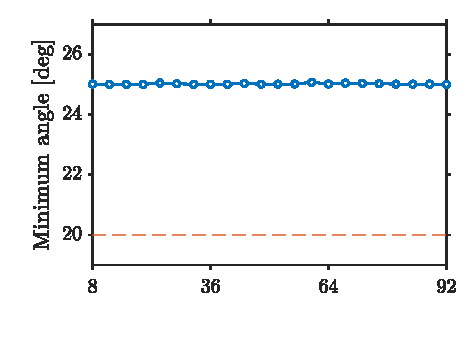
\includegraphics[width=\linewidth]{figures/quality/min_angle.pdf}
    \caption{Minimum triangle-angle check.}
    \label{fig:quality-angle}
  \end{subfigure}
  \hfill
  \begin{subfigure}[t]{0.485\linewidth}
    \centering
    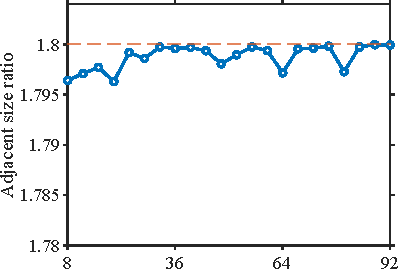
\includegraphics[width=\linewidth]{figures/quality/size_ratio.pdf}
    \caption{Adjacent element-size-ratio check.}
    \label{fig:quality-ratio}
  \end{subfigure}

  \medskip

  \begin{subfigure}[t]{0.485\linewidth}
    \centering
    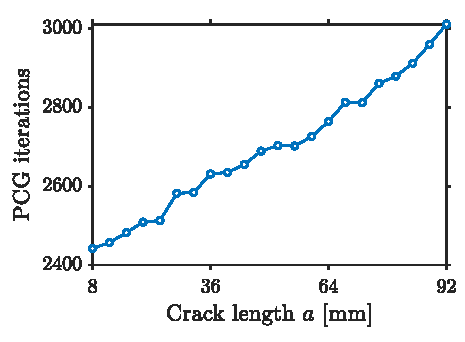
\includegraphics[width=\linewidth]{figures/quality/iterations.pdf}
    \caption{PCG iterations for accepted physical solves.}
    \label{fig:quality-iterations}
  \end{subfigure}
  \hfill
  \begin{subfigure}[t]{0.485\linewidth}
    \centering
    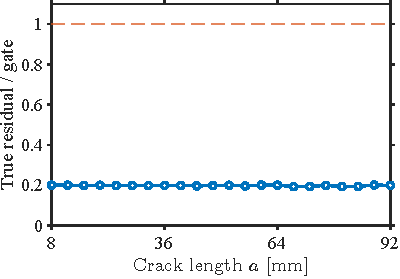
\includegraphics[width=\linewidth]{figures/quality/true_residual.pdf}
    \caption{True relative residual normalized by its acceptance gate.}
    \label{fig:quality-residual}
  \end{subfigure}

  \caption{Diagnostics for accepted $P_2$--$P_{23}$ states. Dashed lines are
  the $20^\circ$ minimum-angle gate, 1.8 adjacent-size-ratio gate, and normalized
  true-residual gate of one. The separately enforced reported-PCG tolerance
  is $10^{-10}$; the true-residual acceptance denominator is
  $5\times10^{-10}$. No failed $P_{24}$ solve is plotted.}
  \label{fig:quality}
\end{figure}

\end{document}
